
\documentclass[11pt]{article}
 
\usepackage[margin=1in]{geometry} 
\usepackage{amsmath,amsthm,amssymb}
\usepackage{graphicx} 
\usepackage{blkarray}
\usepackage{amsmath}




\newcommand{\N}{\mathbb{N}}
\newcommand{\Z}{\mathbb{Z}}
 
\newenvironment{problem}[2][Problem]{\begin{trivlist}
\item[\hskip \labelsep {\bfseries #1}\hskip \labelsep {\bfseries #2.}]}{\end{trivlist}}
\newenvironment{lemma}[2][Lemma]{\begin{trivlist}
\item[\hskip \labelsep {\bfseries #1}\hskip \labelsep {\bfseries #2.}]}{\end{trivlist}}
\newenvironment{exercise}[2][Exercise]{\begin{trivlist}
\item[\hskip \labelsep {\bfseries #1}\hskip \labelsep {\bfseries #2.}]}{\end{trivlist}}

\newenvironment{question}[2][Question]{\begin{trivlist}
\item[\hskip \labelsep {\bfseries #1}\hskip \labelsep {\bfseries #2.}]}{\end{trivlist}}
\newenvironment{corollary}[2][Corollary]{\begin{trivlist}
\item[\hskip \labelsep {\bfseries #1}\hskip \labelsep {\bfseries #2.}]}{\end{trivlist}}

\usepackage{indentfirst}
\linespread{1.2}     % 调整间距
\setlength{\parindent}{0pt}

\begin{document}

 
% --------------------------------------------------------------
%                         Start here
% --------------------------------------------------------------
 
\title{Homework 10 DS-GA 1002 }%replace X with the appropriate number
\author{Yuhao Zhao\\ %replace with your name
Yz3085} %if necessary, replace with your course title
 
\maketitle
\begin{problem}{1}
\end{problem}
a). Let dim(S)=i, and \{$v_1,...,v_i$\} be  a basis of S. Let \{$u_1,...,u_j$\}  be a basis of $S^\perp$.\\
Then $V_i's$ are independent and $u_j's$ are independent.\\
Since $u_m \in S^\perp$ we claim that \{$v_1,...,v_i,u_m$\} are linearly independent.\\

proof:  if $a_1 v_1 + a_2 v_2 + .. +a_i v_i + a_{i+1} u_m = 0$ ,we apply dot product on both side.\\
$a_1 <v_1,u_m> + a_2 <v_2,u_m> + .. +a_i <v_i,u_m> + a_{i+1} <u_m,u_m> = 0$\\
$v_i \perp u_m$, we have $a_{i+1} ||u_m||^2 =0$, hence $a_{i+1} = 0$\\
Then we $a_1 v_1 + a_2 v_2 + .. +a_i v_i  = 0  \to a_1  =a_2 =... = a_i = 0$ \\

Then we can show that \{$v_1,...,v_i,u_1,...u_j$\} are linearly independent. if  i+j $>n$ this contradict to that a n dimension vector space can't have more than n independent vectors. \\
if i+j $<$n, then there exist vector W $\notin $ S and $S^\perp$, this is not possible since by definition, if W $\notin$ S, W $\in S^\perp$. \\

b) Let dim(Null(A)) = r,  \{$u_1,...,u_r$\}  be a a basis for Null(A). \\$\exists$ \{$u_{r+1},...,u_{n}$\} such that \{$u_1,...,u_n$\} is a basis for $R^n$\\
Range(A) = span\{$Au_1,...,Au_n$\} = span\{$0,0,...,Au_{r+1},...,Au_n$\} = span\{$Au_{r+1},...,Au_n$\} \\
We need to prove \{$Au_{r+1},...,Au_n$\}  are linearly independent.\\
$\alpha_{r+1}Au_{r+1}+,...,+\alpha_n Au_n = 0 = A(\alpha_{r+1}u_{r+1}+,...,\alpha_n u_n) $\\
This means $ \alpha_{r+1}u_{r+1}+,...,\alpha_n u_n \in NULL(A)$ thus can be written as linear combination of  \{$u_1,...,u_r$\}\\
$ \alpha_{r+1}u_{r+1}+,...,\alpha_n u_n  = \alpha_1 u_1 + ,..., +\alpha_r u_r$\\
$u_i's$ are linearly independent, we have $\alpha_i's = 0$\\
Then we show that \{$Au_{r+1},...,Au_n$\}  are linearly independent. dim(Range(A)) = n-r\\
Therefore, dim(Null(A))+dim(Range(A))  = n\\

c) Since A is full rank and m $\leq$ n. We know that we can have a singular value decomposition of $A = USV^T$, where the columns of A is a basis for row space of A.\\
Therefore, We know that the projection of X onto row space of A, $P_{row A } X= VV^TX$ \\
Since $A = USV^T$ and $A^T = VSU^T$, $V^T = S^{-1} U^{-1}A$ and $V  = A^T (U^T)^{-1}S^{-1}$ \\
$VV^T = A^T (U^T)^{-1}S^{-1} S^{-1} U^{-1}A$\\
$(AA^T)^{-1} = (US^2U^T)^{-1} = (U^T)^{-1}(S^2)^{-1}U^{-1}$\\
We notice that $VV^T  = A^T(AA^T)^{-1}A$, then we showed that $A^T(AA^T)^{-1}Ax$ is the projection of X on to the row space of X.\\


d) If columns of A are orthonormal and m $\geq $ n, $A^TA = I$  \\
$||y - AA^Ty|| = ||y-y|| = 0$ \\
Since the L2 norm can't be negative, x = $A^T y $ minimize the least-square problem 

\begin{problem}{2}
\end{problem}
a) code:
\begin{verbatim}
index = np.array(list(range(1,n+1)))

d_matrix= np.hstack((np.zeros((n,1))+1,      	
							                     np.transpose([np.cos(2*np.pi*index/12)]),
                     np.transpose([np.sin(2*np.pi*index/12)]),
                     np.transpose([index])))

reconstruction_max = np.dot(d_matrix ,
								                      np.transpose([np.linalg.lstsq(d_matrix,max_temp)[0] ]))
reconstruction_min = np.dot(d_matrix , 
                      np.transpose([np.linalg.lstsq(d_matrix,min_temp)[0] ]))

trend_max =  np.linalg.lstsq(d_matrix,max_temp)[0][-1]*index+
                            np.linalg.lstsq(d_matrix,max_temp)[0][0]
trend_min =  np.linalg.lstsq(d_matrix,min_temp)[0][-1]*index+ 
                            np.linalg.lstsq(d_matrix,min_temp)[0][0]

\end{verbatim}

b) The number of station record positive slope follows a Binomial(100,0.5) distribution, approximately, n $\sim$ N(50, 25) \\
$P(n \geq 65) = P(\frac{n-50}{5} >\frac{65-50}{2}) = P(Z>3) \approx 0.00135$\\

\begin{problem}{3}
\end{problem}
a) Model 1:\\
Since $\vec{w} = \alpha \vec{h}$. The LS solution is $\alpha_{LS} = (h^Th)^{-1}hw$\\
$h^Th = \sum h_i^2, \alpha = \frac{\sum h_iw_i}{\sum h_i^2}$\\

Model 2:\\
Let A = $\begin{bmatrix}
	1 & h_1\\1 &h_2 \\ ...\\ 1 & h_n, 
\end{bmatrix}$ Then w = Ax,\\
 $x_{ls} = (A^TA)^{-1}A^Tw$ = $\begin{bmatrix}
 	n& \sum h_i \\ \sum h_i & \sum h_i^2 
 \end{bmatrix}^{-1} \begin{bmatrix}
 1&1& ... &1\\ h_1 &h_2&...& h_n
 \end{bmatrix} w \\= \frac{1}{n\sum h_i^2 - (\sum h_i)^2}
\begin{bmatrix}
\sum h_i^2 &- \sum h_i \\ -\sum h_i & n
\end{bmatrix} \begin{bmatrix}
1&1& ... &1\\ h_1 &h_2&...& h_n
\end{bmatrix}w$\\
= $\frac{1}{n\sum h_i^2 - (\sum h_i)^2} \begin{bmatrix}
\sum w_i \sum h_i^2 - \sum h_i \sum h_iw_i\\
-\sum w_i \sum h_i + n\sum h_i w_i\\
\end{bmatrix}$\\
therefore, $\alpha = \frac{n\sum h_i w_i -\sum w_i \sum h_i }{n\sum h_i^2 - (\sum h_i)^2}$\\


b)

\begin{centering}
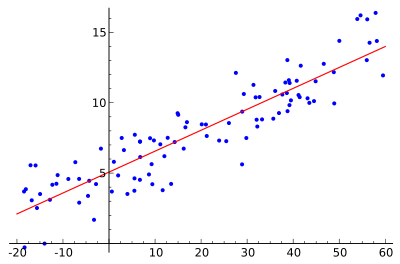
\includegraphics[width = 4in]{q3}\\
\end{centering}

In the data above, it make more sense to include an intercept in the model. Otherwise, the fitted model would go through the origin which is not necessarily true for this data. \\

c)
\begin{verbatim}
Model 1 relative error: 0.0665299568077
Model 2 relative error: 0.0645968638157
\end{verbatim}

d)
\begin{verbatim}
Model 1 relative error: 0.0652793978051
Model 2 relative error: 0.0638616842264
\end{verbatim}
Using 100 training data, we still get very similar relative error rate. For linear models with few  parameters and large data set, adding one more parameter does not change the error rate too much. If we have a lot of data, we should try to fit a more complex model because the over-fitting problem is not significant if the number of parameters are ignorable compared to the number of data. If we don't have enough data, we should try regularized modeling, which may prefer model with less parameters.\\

\begin{problem}{4}
\end{problem}
a) Our target is to minimize the least square error of $Ax-y$\\ Then the solution is given by project y to the column space of A. Using svd we have $A =USV^T$ \\
$x_{ls} = VS^{-1}U^T(y) =VS^{-1}U^T(Ax+z)  = VS^{-1}U^T USV^Tx + VS^{-1}U^Tz = x + VS^{-1}U^Tz$\\

b) $\max\limits_{||z|| = 1} ||x_{ls}-x|| = \max\limits_{||z|| = 1} ||VS^{-1}U^Tz|| = \max\limits_{||z|| = 1} (VS^{-1}U^Tz)^T VS^{-1}U^Tz \\=  \max\limits_{||z|| = 1} z^TUS^{-1}V^TVS^{-1}U^Tz
 = \max\limits_{||z|| = 1} z^TUS^{-2}U^Tz$\\ Let Y = $U^Tz,$, U is an unitary matrix thus preserve vector length $ ||Y|| = 1$\\
 Therefore $\max\limits_{||z|| = 1} z^TUS^{-1}V^TVS^{-1}U^Tz = \max\limits_{||Y|| = 1} Y^T S^{-2}Y$\\
  Since S is a diagonal matrix, the expression is maximized at $\hat{y}$ when $\hat{y}_i = 1$ where i is the ith index such that $\frac{1}{\sigma_i^2}$ is the max and $ \hat{y}_j = 0 $ for all $j\neq i$\\
  $U^T$ is an orthonormal matrix, to make $U^Tz = \hat{y} = \begin{bmatrix}
  0\\...\\1\\...\\0
  \end{bmatrix}$ we just have to select z to be the i-th column of U\\
  In our example, we have A = $\begin{bmatrix}
  2.1&1.1 \\3.2 & 1.6\\ 2.4&1.2
  \end{bmatrix}$\\
  The svd of A is U = $ \begin{bmatrix}
   -0.4.68 &0.884& 0\\
  -0.707& -0.375&  -0.600\\
  -0.530& -0.281&  0.800
  \end{bmatrix}  $ and the corresponding singular values are 5.06146605 and  0.03951424\\
  The max $\frac{1}{\sigma_i^2}$ corresponds to the second one. Therefore our optimal $z = \begin{bmatrix}
  0.884\\-0.375 \\ -0.281
  \end{bmatrix}$\\
  
  c) Let B = $\begin{bmatrix}
  A\\ \gamma I_n
  \end{bmatrix}_{m+n,n}$ and $c = \begin{bmatrix}
  	y\\ \vec{0}_{n\times1}
  \end{bmatrix}_{m+n,1}$\\
  Then $\min\limits_{x} ||Bx -c||_2^2 = \min\limits_{x} ||\begin{bmatrix}
  A\\ \gamma I_n
  \end{bmatrix}x -  \begin{bmatrix}
  y\\ \vec{0}_{n\times1}
  \end{bmatrix} ||^2_2 =  \min\limits_{x} ||\begin{bmatrix}
  Ax\\ \gamma x
  \end{bmatrix} -  \begin{bmatrix}
  y\\ \vec{0}_{n\times1}
  \end{bmatrix} ||^2_2 \\ =  \min\limits_{x} ||\begin{bmatrix}
  Ax - y\\ \gamma x
  \end{bmatrix}  ||^2_2 =  \min\limits_{x}  ||Ax-y||^2_2 + \gamma^2 ||x||^2_2 $\\
  \pagebreak
  
  d) Our target is to minimize $||Ax-y||^2_2 + \gamma^2 ||x||^2_2 $\\
  Using Lagrange Multiplier, this is equivalent to  $\min\limits_{x}  ||Ax-y||^2_2$ subject to $\sum x_i^2 \leq \tau$\\
  The problem can be solved by taking derivative, $\nabla_x ( ||Ax-y||^2_2 + \gamma^2 ||x||^2_2) = 0$ \\
$\nabla_x ( ||Ax-y||^2_2 + \gamma^2 ||x||^2_2) = 2A^T(Ax-y)+2\gamma^2 I_n x = 0\\ A^TAx +\gamma^2 I_n x- A^Ty = 0\\$ Then, $ x_{rr} = (A^TA+\gamma^2 I_n)^{-1} A^Ty $\\
	
Now using svd of $A = USV^{-1}$\\
$A^TA = (USV^T)^TUSV^T = VS^TU^TUSV^T = VS^2V^T\\
x_{rr} =  (VS^2V^T +\gamma^2 I_n)^{-1}VSU^Ty, \text{ since } \gamma^2I_n = \gamma^2VI_nV^T\\
RHS = (V(S^2+\gamma^2I_n)V^T)^{-1}VSU^Ty =V(S^2+\gamma^2I_n)^{-1}V^TVSU^T(Ax+z)\\ = V(S^2+\gamma^2I_n)^{-1}S^2V^Tx+  V(S^2+\gamma^2I_n)^{-1} SU^Tz\\
(S^2+\gamma^2I_n)^{-1} = \begin{bmatrix}
\frac{1}{\sigma_1^2 + \gamma^2}&0&0 &...&0\\0& \frac{1}{\sigma_2^2+\gamma^2}&0&...&0\\
& ...\\0&0&...&0&\frac{1}{\sigma_m^2 +\gamma^2}
\end{bmatrix}$\\
RHS = $\begin{bmatrix}
v_1 \frac{1}{\sigma_1^2 + \gamma^2}, v_2 \frac{1}{\sigma_2^2 + \gamma^2},... , v_m\frac{1}{\sigma_m^2 + \gamma^2}
\end{bmatrix}(S^2V^Tx +SU^TZ )\\ = \sum \frac{\sigma_i^2}{\sigma_i^2 + \gamma^2} v_i^Txv_i + \sum \frac{\sigma_i}{\sigma_i^2 + \gamma^2}  u_i^Tzv_i $\\

e) $x_{rr} - x = \sum \frac{\sigma_i^2}{\sigma_i^2 + \gamma^2} v_i^Txv_i + \sum \frac{\sigma_i}{\sigma_i^2 + \gamma^2}  u_i^Tzv_i  - x$\\
Since $VV^T = I$\\
RHS$ = \sum \frac{\sigma_i^2}{\sigma_i^2 + \gamma^2} v_i^Txv_i + \sum \frac{\sigma_i}{\sigma_i^2 + \gamma^2}  u_i^Tzv_i  - \sum  v_i^Tv_ix \\=
\sum \frac{-\gamma^2}{\sigma_i^2 + \gamma^2} v_i^Tv_ix  + \sum \frac{\sigma_i}{\sigma_i^2 + \gamma^2}  u_i^Tzv_i $\\
We notice that the norm of the left expression increases as $\gamma$ increases. and the right expression decreases as $\gamma$ increases\\

f) For matrix that is badly conditioned, it has some very small singular values. For the least square regression, the solution to the system of equations becomes very susceptible to noise in the data. However, the Ridge is rather stable. For the small singular values, the corresponding $x_{rr}$ expression becomes closed to $\lim\limits_{\sigma_i \to 0} \frac{-\gamma^2}{\sigma_i^2 + \gamma^2} v_i^Tv_ix  + \frac{\sigma_i}{\sigma_i^2 + \gamma^2}  u_i^Tzv_i  = -v_i^Tv_ix $ which is not  very large. This helps to control the error. For regular matrix, the regulation won't have a big influence on the exact solution.  




\end{document}